\pagebreak
\begin{frame}{Grundlegende Theorie}{Definition}
    Im weitesten Sinne beschreibt ein Buffer Overflow eine Schwachstelle in einem Computerprogramm,
    bei der ein Angreifer einen Speicherbereich fester Größe überschreibt und diesen so zum “Überlaufen” bringt.
    Durch Ausspähen und Analysieren der Software kann dieses Überschreiben so gezielt geschehen, dass der Fluss des
    Programms verändert und zuvor injizierter Schadcode ausgeführt wird.    
\end{frame}


\begin{frame}{Grundlegende Theorie}{Speicheraufbau}
    \begin{figure}[h]
        \centering
        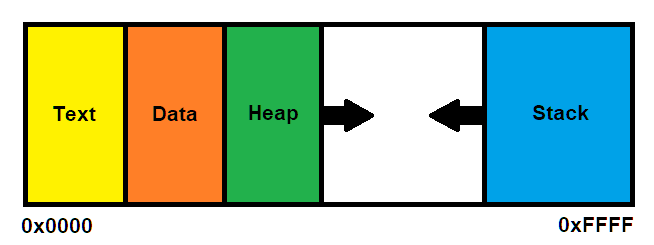
\includegraphics[width=0.7\textwidth,height=0.75\textheight,keepaspectratio]{images/process.png}
        \caption{Prozess im Speicher}
    \end{figure}
\end{frame}

\begin{frame}{Grundlegende Theorie}{Stack Overflow}
    \begin{itemize}
        \setlength{\itemindent}{19em}
        \item Wert einer Variable verändern
        \item Function Pointer manipulieren
        \item Return Pointer überschreiben        
    \end{itemize}
    \begin{figure}[h]
        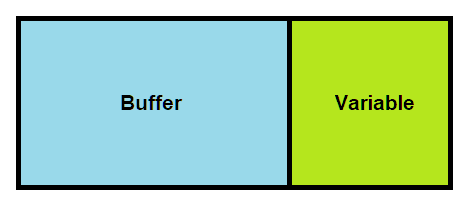
\includegraphics[width=0.475\textwidth]{images/buffer1.png}
        \hfill
        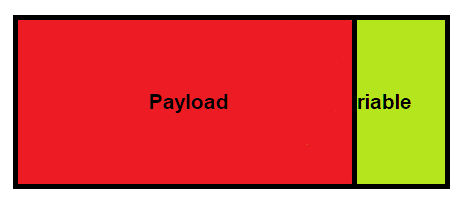
\includegraphics[width=0.475\textwidth]{images/buffer2.png}
        \caption{Buffer im Stack während eines Overflows}
    \end{figure}
\end{frame}



\begin{frame}{Grundlegende Theorie}{Heap Overflow}
Während der Laufzeit eines Programms allozierter Speicher (z.\,B. durch \codeline{malloc()}) wird im Heap angelegt. Dabei setzt sich
jeder Speicherblock aus einem Header und dem tatsächlich angeforderten Speicher zusammen. Der Header enthält hierbei,
je nach Implementation, Informationen über den Block, wie z.\,B. seine Größe. Aus diesen Informationen kann dann abgeleitet
werden, an welcher Stelle der nächste Block beginnt.
\end{frame}



